\documentclass[aspectratio=169,10pt]{beamer}
% Shared preamble for the main deck and the backup deck.
% Compile with lualatex (see README.md).
\usetheme[progressbar=frametitle,numbering=fraction,sectionpage=progressbar]{metropolis}
\usepackage{fontspec}
\usepackage{unicode-math}
\setsansfont{Fira Sans}[BoldFont={Fira Sans SemiBold}, ItalicFont={Fira Sans Italic}, BoldItalicFont={Fira Sans SemiBold Italic}]
\setmonofont{Fira Mono}[Scale=0.9]
\setmathfont{Fira Math}
\usepackage{tikz}
\usetikzlibrary{arrows.meta,positioning,calc,shapes.geometric,fit,backgrounds,decorations.pathreplacing}
\usepackage{pgfplots}
\pgfplotsset{compat=1.18}
\usepackage{booktabs}
\usepackage{tabularx}
\usepackage{array}
\usepackage{xcolor}
\usepackage{fontawesome5}

% ---- palette -------------------------------------------------------------
\definecolor{ink}{HTML}{1F2A3A}      % text
\definecolor{navy}{HTML}{23395B}     % frame titles
\definecolor{blue}{HTML}{2F6DB5}     % main data colour (history, popular, known)
\definecolor{teal}{HTML}{1F8A70}     % method / good
\definecolor{orange}{HTML}{D9622B}   % cold start / warning / target
\definecolor{sand}{HTML}{F3EEE6}     % boxes
\definecolor{mist}{HTML}{E8EEF5}     % light blue boxes
\definecolor{grey}{HTML}{7A8494}

\setbeamercolor{normal text}{fg=ink,bg=white}
\setbeamercolor{frametitle}{bg=navy,fg=white}
\setbeamercolor{progress bar}{fg=orange,bg=navy!40}
\setbeamercolor{alerted text}{fg=orange}
\setbeamercolor{example text}{fg=teal}
\setbeamercolor{title separator}{fg=orange}
\metroset{block=fill}
\setbeamercolor{block title}{bg=mist,fg=navy}
\setbeamercolor{block body}{bg=mist!45,fg=ink}
\setbeamerfont{bibliography item}{size=\scriptsize}
\setbeamerfont{bibliography entry author}{size=\scriptsize}
\setbeamerfont{bibliography entry title}{size=\scriptsize}
\setbeamerfont{bibliography entry location}{size=\scriptsize}
\setbeamerfont{bibliography entry note}{size=\scriptsize}
\setbeamercolor{bibliography item}{fg=navy}
\setbeamercolor{bibliography entry author}{fg=ink}
\setbeamercolor{bibliography entry title}{fg=ink}
\setbeamercolor{bibliography entry location}{fg=ink}
\setbeamercolor{footnote}{fg=grey}
\setbeamerfont{footnote}{size=\tiny}
\setbeamerfont{frametitle}{size=\large}
\setbeamertemplate{itemize item}{\color{orange}\textbullet}
\setbeamertemplate{itemize subitem}{\color{grey}--}
\setlength{\leftmargini}{1.1em}

% ---- helpers ---------------------------------------------------------------
\newcommand{\code}[1]{\texttt{#1}}
% source line at the bottom of a frame
\newcommand{\source}[1]{\par\vfill\hfill{\scriptsize\color{grey}#1}}
% big number tile: \stat{value}{label}
\newcommand{\stat}[2]{%
  \begin{tikzpicture}
    \node[fill=mist,rounded corners=3pt,minimum width=2.55cm,minimum height=1.75cm,align=center,inner sep=4pt]
      {{\Large\bfseries\color{navy}#1}\\[2pt]{\scriptsize\color{ink}#2}};
  \end{tikzpicture}}
% one-line takeaway box at the bottom of a slide
\newcommand{\takeaway}[1]{%
  \par\vspace{4pt}\noindent
  \begin{tikzpicture}
    \node[fill=sand,draw=orange,line width=0.6pt,rounded corners=3pt,text width=0.92\textwidth,inner sep=6pt,align=left]
      {\small\textbf{\color{orange}Takeaway.} #1};
  \end{tikzpicture}}
\newcommand{\done}{{\color{teal}\faCheckCircle\ done}}
\newcommand{\planned}{{\color{orange}\faClock[regular]\ planned}}

\tikzset{
  box/.style={draw=navy,rounded corners=3pt,fill=mist,align=center,inner sep=4pt,font=\small},
  arr/.style={-{Stealth[length=2.2mm]},thick,color=navy},
  tok/.style={circle,draw=navy,thick,minimum size=7mm,inner sep=0pt,font=\scriptsize\bfseries},
  user/.style={rectangle,align=center,rounded corners=2pt,draw=grey,fill=white,minimum size=6mm,inner sep=1pt,font=\scriptsize},
}

\title{Next-Token Recommendation for Decentralized-Exchange Traders}
\author{Gergely Madarász \and Levente Tóth \and Béla Jakab}
\institute{Budapest University of Technology and Economics\\Advanced Machine Learning, project plan}
\date{October 2026}

\subtitle{A project plan}

\begin{document}

% ===========================================================================
\maketitle

% ---------------------------------------------------------------------------
\begin{frame}{The question in one sentence}
  \begin{center}
    \Large\color{navy}
    Given what a trader has bought and sold so far,\\
    which \textbf{new} token will it trade in the \textbf{next two days}?
  \end{center}
  \vspace{6pt}
  \begin{columns}[T]
    \begin{column}{0.47\textwidth}
      \textbf{What this talk covers}
      \begin{enumerate}\small
        \item The setting, explained from zero
        \item What the literature says
        \item The data
        \item Preprocessing and the train/dev/test split
        \item The baseline, the metric and the protocol
        \item The proposed method and why it fits
        \item Work plan, risks, limitations
      \end{enumerate}
    \end{column}
    \begin{column}{0.47\textwidth}
      \textbf{What is done and what is not}
      \begin{itemize}\small
        \item \done: data of 14 days, preprocessing, split, a fixed baseline with results
        \item \planned: more data (12 weeks), the models, the test
        \item \alert{No model results are claimed in this talk.}
      \end{itemize}
    \end{column}
  \end{columns}
\end{frame}

% ===========================================================================
\section{The setting, from zero}

\begin{frame}{Four words we need: token, exchange, pool, swap}
  \begin{columns}[c]
    \begin{column}{0.48\textwidth}
      \begin{itemize}\small
        \item \textbf{Token:} a digital asset on the Ethereum blockchain. There are tens of thousands (e.g.\ USDC, LINK, PEPE).
        \item \textbf{Decentralized exchange (DEX):} a program on the blockchain where anyone can trade tokens. We use Uniswap V2/V3 and copies of it.
        \item \textbf{Pool:} a reserve of \emph{two} tokens. You put one token in and take the other out.
        \item \textbf{Swap:} one such trade. Every swap is recorded publicly, with the \textbf{account} (address) that signed it.
      \end{itemize}
    \end{column}
    \begin{column}{0.5\textwidth}
      \centering
      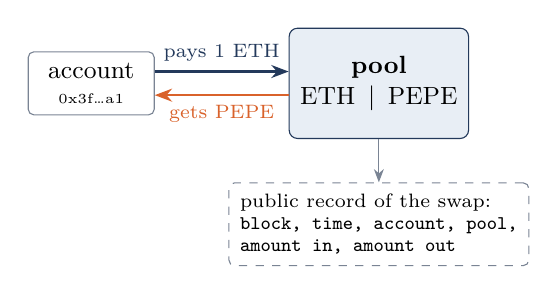
\begin{tikzpicture}[node distance=1.0cm]
        \node[user,minimum width=1.6cm,minimum height=8mm,font=\small] (u) {account\\[-2pt]\tiny 0x3f…a1};
        \node[box,right=1.7cm of u,minimum width=2.2cm,minimum height=1.4cm] (p) {\textbf{pool}\\ ETH \,|\, PEPE};
        \draw[arr] ($(u.east)+(0,0.15)$) -- node[above,font=\scriptsize]{pays 1 ETH} ($(p.west)+(0,0.15)$);
        \draw[arr,orange] ($(p.west)+(0,-0.15)$) -- node[below,font=\scriptsize]{gets PEPE} ($(u.east)+(0,-0.15)$);
        \node[below=0.55cm of p,draw=grey,dashed,rounded corners=2pt,font=\scriptsize,align=left,inner sep=4pt,fill=white] (rec)
          {public record of the swap:\\ \code{block, time, account, pool,}\\ \code{amount in, amount out}};
        \draw[grey,-{Stealth}] (p) -- (rec);
      \end{tikzpicture}
    \end{column}
  \end{columns}
  \takeaway{Every trade of every account is public. This gives us a large, free log of who traded what, and when.}
\end{frame}

\begin{frame}{This is a recommendation problem}
  \begin{columns}[c]
    \begin{column}{0.5\textwidth}
      \small
      A recommender ranks \emph{items} for each \emph{user}, like films on Netflix.
      \begin{center}
      \begin{tabular}{@{}lll@{}}
        \toprule
                  & Netflix & Our project \\
        \midrule
        user      & viewer  & trading account \\
        item      & film    & token \\
        signal    & watched & traded \\
        \bottomrule
      \end{tabular}
      \end{center}
      \textbf{Implicit feedback:} we only see what an account \emph{did} trade.
      Not trading a token does not mean dislike; we have no ratings and no negatives \cite{hu2008,rendle2009}.
    \end{column}
    \begin{column}{0.46\textwidth}
      \centering
      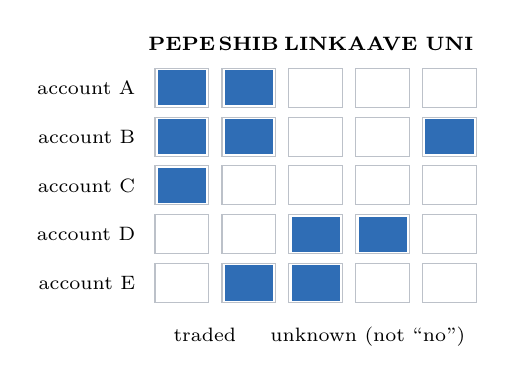
\begin{tikzpicture}[x=0.85cm,y=0.62cm]
        \foreach \t [count=\i] in {PEPE,SHIB,LINK,AAVE,UNI} \node[font=\scriptsize\bfseries,rotate=0] at (\i,0.9) {\t};
        \foreach \u [count=\j] in {A,B,C,D,E} \node[font=\scriptsize,anchor=east] at (0.45,-\j+1) {account \u};
        \foreach \i/\j in {1/1,2/1,1/2,2/2,1/3,3/4,4/4,2/5,3/5,5/2} \fill[blue] (\i-0.36,-\j+1-0.36) rectangle (\i+0.36,-\j+1+0.36);
        \foreach \i in {1,...,5} \foreach \j in {1,...,5} \draw[grey!50] (\i-0.4,-\j+1-0.4) rectangle (\i+0.4,-\j+1+0.4);
        \node[font=\scriptsize,align=center] at (3,-5.1) {\textcolor{blue}{$\blacksquare$} traded \quad $\square$ unknown (not ``no'')};
      \end{tikzpicture}
      \par\scriptsize\color{grey} Toy example. In the real data only 0.014\% of the cells are filled.
    \end{column}
  \end{columns}
\end{frame}

\begin{frame}{What exactly is predicted: one evaluation point}
  \centering
  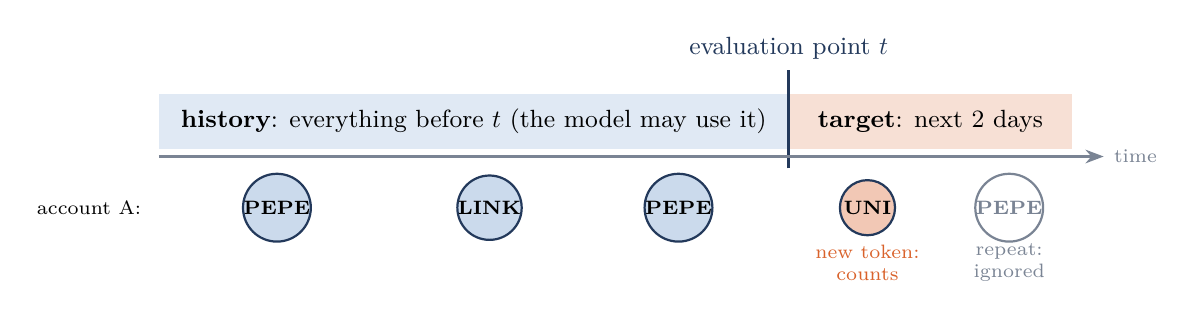
\begin{tikzpicture}[x=1cm,y=1cm]
    \fill[blue!15] (0,0) rectangle (8,0.7);
    \fill[orange!20] (8,0) rectangle (11.6,0.7);
    \node[font=\small] at (4,0.35) {\textbf{history}: everything before $t$ (the model may use it)};
    \node[font=\small] at (9.8,0.35) {\textbf{target}: next 2 days};
    \draw[very thick,navy] (8,-0.25) -- (8,1.0) node[above,font=\small] {evaluation point $t$};
    \draw[-{Stealth},thick,grey] (0,-0.1) -- (12.0,-0.1) node[right,font=\scriptsize] {time};
    % example account
    \node[font=\scriptsize,anchor=east] at (-0.1,-0.75) {account A:};
    \foreach \x/\l in {1.5/PEPE,4.2/LINK,6.6/PEPE} \node[tok,fill=blue!25] at (\x,-0.75) {\l};
    \node[tok,fill=orange!35] at (9.0,-0.75) {UNI};
    \node[tok,fill=white,draw=grey] at (10.8,-0.75) {\textcolor{grey}{PEPE}};
    \node[font=\scriptsize,orange,align=center] at (9.0,-1.45) {new token:\\counts};
    \node[font=\scriptsize,grey,align=center] at (10.8,-1.45) {repeat:\\ignored};
  \end{tikzpicture}
  \vspace{4pt}
  \begin{enumerate}\small
    \item At time $t$, for every account, rank all tokens it has \textbf{never} traded before $t$.
    \item Show the top 10.
    \item A \textbf{hit} is a token in the list that the account trades for the first time in the two days after $t$.
  \end{enumerate}
  \takeaway{The labels come from the blockchain itself: exact, free, and available for any period.}
\end{frame}

% ===========================================================================
\section{What the literature says}

\begin{frame}{The literature in four groups (21 references)}
  \small
  \begin{columns}[T]
    \begin{column}{0.49\textwidth}
      \begin{block}{1. Recommending from implicit feedback}
        Weighted matrix factorization \cite{hu2008}; ranking loss \cite{rendle2009};
        \textbf{item-based nearest neighbours} \cite{sarwar2001};
        top-$N$ evaluation \cite{cremonesi2010}; linear item model \cite{steck2019}; short sessions \cite{hidasi2016}.
      \end{block}
      \begin{block}{2. Simple methods are hard to beat}
        Many neural recommenders lose to tuned simple ones \cite{dacrema2019,rendle2020,rendle2021,anelli2022,ludewig2018};
        popularity is a strong baseline when measured at the right time \cite{li2021,ji2020pop}.
      \end{block}
    \end{column}
    \begin{column}{0.49\textwidth}
      \begin{block}{3. Evaluating without fooling yourself}
        Per-user splits leak the future \cite{ji2020leak}; the split changes conclusions \cite{meng2020};
        sampled metrics mislead \cite{krichene2020}; new items need content \cite{schein2002}.
      \end{block}
      \begin{block}{4. Ranking and on-chain assets}
        Learning to rank \cite{burges2010}; two-stage systems \cite{covington2016};
        NFT recommenders \cite{choi2024,nftmine2023}.
      \end{block}
    \end{column}
  \end{columns}
\end{frame}

% ===========================================================================
\section{The data}

\begin{frame}{The dataset of the feasibility study \hfill \done}
  \centering
  \stat{14 days}{24 Sep -- 8 Oct 2026}\hspace{4pt}
  \stat{2.71 M}{swaps}\hspace{4pt}
  \stat{211{,}547}{accounts}\hspace{4pt}
  \stat{20{,}014}{tokens}\hspace{4pt}
  \stat{440 MB}{on disk}
  \vspace{8pt}
  \begin{columns}[T]
    \begin{column}{0.48\textwidth}
      \small
      \textbf{Source.} Every swap on Uniswap V2/V3-style pools on Ethereum, read from free public endpoints. No key, no licence restriction.
      \par\medskip
      \textbf{One row per swap:} block, time, signing account, pool, amounts. The signs of the amounts tell what was paid and what was received.
    \end{column}
    \begin{column}{0.48\textwidth}
      \small
      \textbf{Validation.}
      \begin{itemize}
        \item no duplicate events, no missing values
        \item 99.1\% of blocks contain a swap
        \item tokens known for 99.98\% of swaps
        \item 164k--225k swaps on each full day
      \end{itemize}
    \end{column}
  \end{columns}
\end{frame}

\begin{frame}{The data is very sparse and very skewed}
  \begin{columns}[c]
    \begin{column}{0.52\textwidth}
      \centering
      {\small\bfseries How many tokens does an account trade?}\par\smallskip
      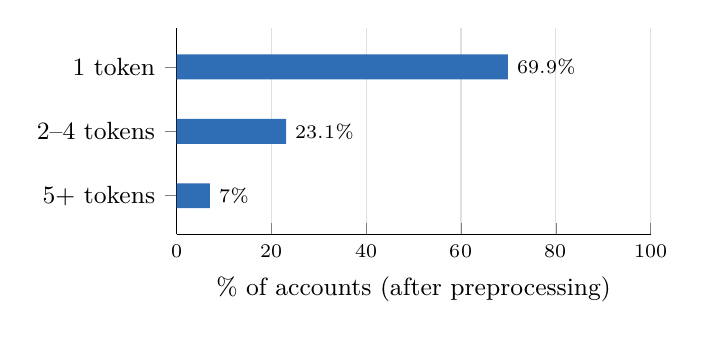
\begin{tikzpicture}
        \begin{axis}[
          width=7.6cm,height=4.2cm,
          xbar, bar width=9pt, xmin=0, xmax=100,
          symbolic y coords={{5+ tokens},{2--4 tokens},{1 token}},
          ytick=data, y tick label style={font=\small},
          xlabel={\% of accounts (after preprocessing)}, xlabel style={font=\small},
          tick label style={font=\scriptsize},
          nodes near coords={\pgfmathprintnumber{\pgfplotspointmeta}\%}, nodes near coords style={font=\scriptsize},
          axis lines*=left, enlarge y limits=0.3, xmajorgrids, grid style={grey!25},
        ]
          \addplot[fill=blue,draw=none] coordinates {(7,{5+ tokens}) (23.1,{2--4 tokens}) (69.9,{1 token})};
        \end{axis}
      \end{tikzpicture}
      \par\scriptsize\color{grey} 157{,}060 accounts: 47{,}280 with $\geq$2 tokens, 11{,}000 with $\geq$5.
    \end{column}
    \begin{column}{0.44\textwidth}
      \small
      \begin{itemize}
        \item The account--token table is \textbf{0.014\%} full.
        \item The \textbf{typical account trades one token}.
        \item The 10 most used pools carry \textbf{29\%} of all swaps.
        \item The 1{,}000 most active accounts make \textbf{57\%} of all swaps (many are bots).
      \end{itemize}
    \end{column}
  \end{columns}
  \takeaway{Many events, but few accounts with enough history to personalize for. Popularity will be a strong reference.}
\end{frame}

% ===========================================================================
\section{Preprocessing and split}

\begin{frame}{The central decision: the item is the token, not the pool}
  \centering
  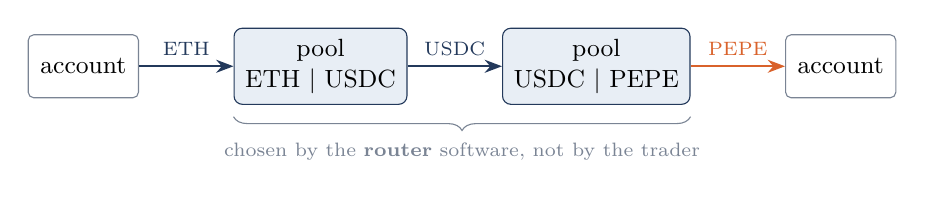
\begin{tikzpicture}[node distance=1.1cm]
    \node[user,minimum width=1.4cm,minimum height=8mm,font=\small] (u) {account};
    \node[box,right=1.2cm of u,minimum width=2.0cm] (p1) {pool\\ETH | USDC};
    \node[box,right=1.2cm of p1,minimum width=2.0cm] (p2) {pool\\USDC | PEPE};
    \node[user,right=1.2cm of p2,minimum width=1.4cm,minimum height=8mm,font=\small] (u2) {account};
    \draw[arr] (u) -- node[above,font=\scriptsize]{ETH} (p1);
    \draw[arr] (p1) -- node[above,font=\scriptsize]{USDC} (p2);
    \draw[arr,orange] (p2) -- node[above,font=\scriptsize]{PEPE} (u2);
    \draw[decorate,decoration={brace,amplitude=5pt,mirror},grey] ($(p1.south west)+(0,-0.15)$) -- ($(p2.south east)+(0,-0.15)$)
      node[midway,below=6pt,font=\scriptsize,grey] {chosen by the \textbf{router} software, not by the trader};
  \end{tikzpicture}
  \vspace{2pt}
  \begin{columns}[T]
    \begin{column}{0.49\textwidth}
      \small
      \begin{itemize}
        \item 20\% of transactions pass through more than one pool.
        \item Of the ``new pools'' an account touches, only 73\% are a token new to it.
      \end{itemize}
    \end{column}
    \begin{column}{0.49\textwidth}
      \small
      \textbf{So:} each transaction is reduced to what the account finally \emph{sold} (ETH) and \emph{bought} (PEPE).
      USDC was only passed through and is dropped.
    \end{column}
  \end{columns}
  \takeaway{The trader chooses the token; software chooses the pools. We model the trader's choice.}
\end{frame}

\begin{frame}{Other preprocessing decisions \hfill \done}
  \small
  \renewcommand{\arraystretch}{1.3}
  \begin{tabularx}{\textwidth}{@{}>{\raggedright\arraybackslash}p{5.2cm}>{\raggedright\arraybackslash}X@{}}
    \toprule
    What we found in the data & What we do \\
    \midrule
    Base currencies are in almost every trade (WETH 81\% of accounts, USDC 40\%, USDT 29\%; next token: 5\%) & Remove tokens traded by $>$10\% of accounts. Decided on the training period only. \\
    Arbitrage bots trade in cycles that end where they start & Such cycles leave no bought or sold token and drop out by themselves. \\
    A few accounts make thousands of swaps & Interactions are binary (traded or not); every metric is an average over accounts. \\
    Half of next trades are repeats & Only \emph{new} tokens are the target. \\
    Some target tokens did not exist yet at time $t$ & Kept, and counted as misses. Scores reflect the real task. \\
    \bottomrule
  \end{tabularx}
  \source{Result: 157{,}060 accounts, 19{,}631 tokens, median 1 token per account.}
\end{frame}

\begin{frame}{The split: one global timeline}
  \small
  \textbf{Rule.} At an evaluation point $t$, \emph{all} accounts share the same cut. Points are grouped into periods by calendar date.
  \par\vspace{6pt}
  \begin{center}
  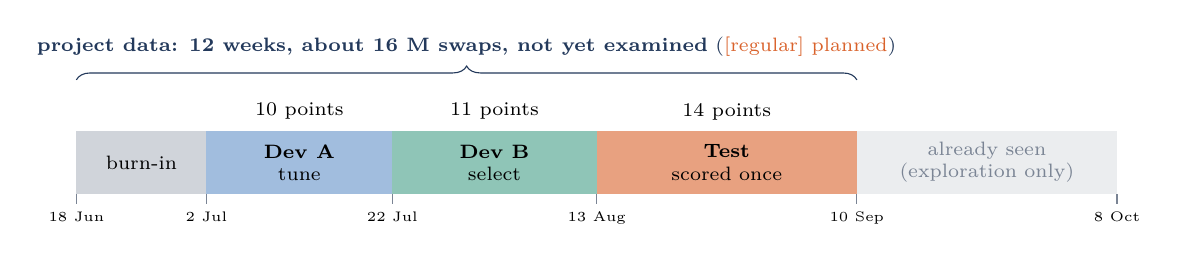
\begin{tikzpicture}[x=0.118cm,y=1cm]
    % days from 18 June (day 0) to 8 Oct (day 112)
    \fill[grey!35]  (0,0) rectangle (14,0.8);
    \fill[blue!45]  (14,0) rectangle (34,0.8);
    \fill[teal!50]  (34,0) rectangle (56,0.8);
    \fill[orange!60](56,0) rectangle (84,0.8);
    \fill[grey!15]  (84,0) rectangle (112,0.8);
    \node[font=\scriptsize,align=center] at (7,0.4) {burn-in};
    \node[font=\scriptsize,align=center] at (24,0.4) {\textbf{Dev A}\\tune};
    \node[font=\scriptsize,align=center] at (45,0.4) {\textbf{Dev B}\\select};
    \node[font=\scriptsize,align=center] at (70,0.4) {\textbf{Test}\\scored once};
    \node[font=\scriptsize,align=center,grey] at (98,0.4) {already seen\\(exploration only)};
    \foreach \x/\d in {0/18 Jun,14/2 Jul,34/22 Jul,56/13 Aug,84/10 Sep,112/8 Oct}
      {\draw[grey] (\x,0) -- (\x,-0.12); \node[font=\tiny,below] at (\x,-0.1) {\d};}
    \node[font=\scriptsize] at (24,1.05) {10 points};
    \node[font=\scriptsize] at (45,1.05) {11 points};
    \node[font=\scriptsize] at (70,1.05) {14 points};
    \draw[decorate,decoration={brace,amplitude=5pt},navy] (0,1.45) -- (84,1.45) node[midway,above=5pt,font=\scriptsize,navy] {\textbf{project data: 12 weeks, about 16 M swaps, not yet examined} (\planned)};
  \end{tikzpicture}
  \end{center}
  \begin{itemize}
    \item Each point: history = everything before it; target = the next 2 days. Targets do \textbf{not overlap}.
    \item Order is chronological: tune $\rightarrow$ select $\rightarrow$ test. Test is scored \textbf{once}, from a frozen commit.
    \item Honest caveat: the test period is untouched, but it lies \emph{before} the data we explored.
  \end{itemize}
\end{frame}

\begin{frame}{Why not a random split? Leakage}
  \begin{columns}[T]
    \begin{column}{0.5\textwidth}
      \centering
      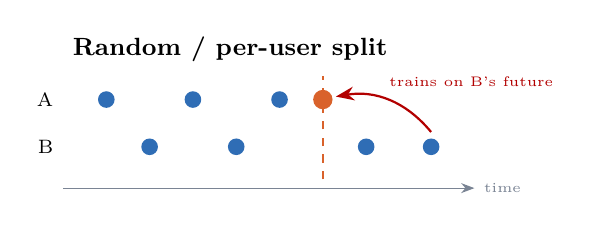
\begin{tikzpicture}[x=0.55cm,y=0.75cm]
        \node[font=\small\bfseries,anchor=west] at (0,2.35) {Random / per-user split};
        \draw[-{Stealth},grey] (0,0) -- (9.5,0) node[right,font=\tiny] {time};
        \node[font=\scriptsize,anchor=east] at (0,1.5) {A};
        \node[font=\scriptsize,anchor=east] at (0,0.7) {B};
        \foreach \x in {1,3,5} \fill[blue] (\x,1.5) circle (3pt);
        \fill[orange] (6,1.5) circle (3.5pt);
        \foreach \x in {2,4,7,8.5} \fill[blue] (\x,0.7) circle (3pt);
        \draw[orange,thick,dashed] (6,0.15) -- (6,1.9);
        \draw[red!70!black,-{Stealth},thick] (8.5,0.95) to[bend right=30] node[above right,font=\tiny,red!70!black,pos=0.6]{trains on B's future} (6.3,1.55);
      \end{tikzpicture}
      \par\vspace{6pt}
      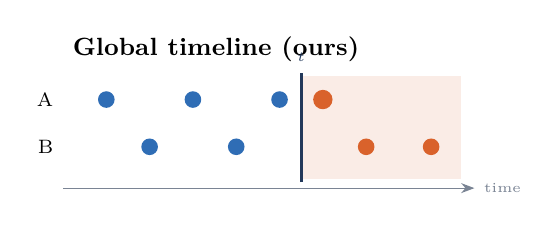
\begin{tikzpicture}[x=0.55cm,y=0.75cm]
        \node[font=\small\bfseries,anchor=west] at (0,2.35) {Global timeline (ours)};
        \draw[-{Stealth},grey] (0,0) -- (9.5,0) node[right,font=\tiny] {time};
        \node[font=\scriptsize,anchor=east] at (0,1.5) {A};
        \node[font=\scriptsize,anchor=east] at (0,0.7) {B};
        \fill[orange!12] (5.5,0.15) rectangle (9.2,1.9);
        \foreach \x in {1,3,5} \fill[blue] (\x,1.5) circle (3pt);
        \fill[orange] (6,1.5) circle (3.5pt);
        \foreach \x in {2,4} \fill[blue] (\x,0.7) circle (3pt);
        \foreach \x in {7,8.5} \fill[orange] (\x,0.7) circle (3pt);
        \draw[navy,very thick] (5.5,0.1) -- (5.5,1.95) node[above,font=\tiny] {$t$};
      \end{tikzpicture}
    \end{column}
    \begin{column}{0.47\textwidth}
      \small
      \textbf{Leakage} = the model sees information it could not have had at prediction time \cite{ji2020leak}.
      \par\medskip
      \textbf{Main controls}
      \begin{itemize}
        \item one cut in time for all accounts
        \item token statistics only from the history
        \item base-currency list fixed on training days
        \item settings on Dev A, choice on Dev B, test once
        \item ranker validated on held-out \emph{points}
      \end{itemize}
    \end{column}
  \end{columns}
  \source{Full list of 13 risks and controls: backup slides.}
\end{frame}

% ===========================================================================
\section{Baseline, metric and protocol}

\begin{frame}{The metric: recall@10, on a small example}
  \begin{columns}[c]
    \begin{column}{0.44\textwidth}
      \centering
      \begin{tikzpicture}[y=0.42cm]
        \node[font=\scriptsize\bfseries] at (1.1,0.9) {list for account A};
        \foreach \t [count=\i] in {MOG,UNI,LINK,ONDO,PEPE2,AAVE,ENA,SPX,LDO,TURBO} {
          \node[font=\tiny,grey,anchor=east] at (0,-\i+1) {\i};
          \ifnum\i=2 \node[fill=orange!35,draw=orange,minimum width=2.2cm,minimum height=0.36cm,font=\scriptsize,anchor=west,inner sep=1pt] at (0.05,-\i+1) {\t\ \ \faCheck};
          \else \node[fill=mist,minimum width=2.2cm,minimum height=0.36cm,font=\scriptsize,anchor=west,inner sep=1pt] at (0.05,-\i+1) {\t}; \fi
        }
        \node[font=\scriptsize\bfseries,align=center] at (4.0,0.9) {A actually picks up};
        \node[fill=orange!35,draw=orange,font=\scriptsize,minimum width=1.5cm] at (4.0,-1) {UNI};
        \node[fill=white,draw=grey,font=\scriptsize,minimum width=1.5cm] at (4.0,-2.2) {WOJAK};
        \node[fill=white,draw=grey,font=\scriptsize,minimum width=1.5cm] at (4.0,-3.4) {NEWCOIN};
        \node[font=\tiny,orange,align=center] at (4.0,-4.6) {(launched after $t$:\\ unreachable)};
      \end{tikzpicture}
      \par\scriptsize\color{grey} Token names: illustration only.
    \end{column}
    \begin{column}{0.53\textwidth}
      \small
      \[
        \text{recall@10}(A) = \frac{|\text{list} \cap \text{picked up}|}{|\text{picked up}|} = \frac{1}{3}
      \]
      Then average over all evaluated accounts.
      \begin{itemize}
        \item \textbf{Why 10:} a person can read a short list.
        \item \textbf{Why average over accounts:} a bot with 10{,}000 swaps counts as much as a person with 2.
        \item \textbf{Also reported:} NDCG@10 (rewards hits near the top), hit rate (share of accounts with $\geq$1 hit), coverage (share of tokens ever shown).
      \end{itemize}
    \end{column}
  \end{columns}
\end{frame}

\begin{frame}{The fixed baseline: ``the 10 most popular tokens''}
  \small
  \textbf{Popularity:} rank tokens by how many distinct accounts traded them in the history; skip the account's own.
  No settings; the same list for everyone; measured at time $t$ \cite{ji2020pop}.
  \begin{columns}[c]
    \begin{column}{0.6\textwidth}
      \centering
      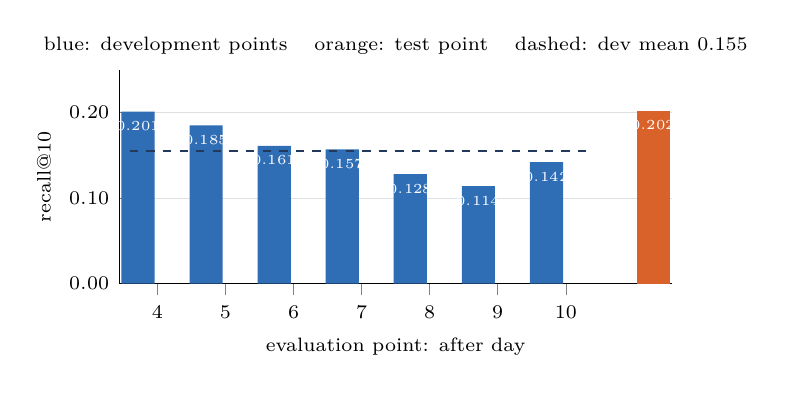
\begin{tikzpicture}
        \begin{axis}[
          width=8.6cm,height=4.3cm, ybar, bar width=12pt,
          ymin=0, ymax=0.25,
          symbolic x coords={d4,d5,d6,d7,d8,d9,d10,d12},
          xticklabels={4,5,6,7,8,9,10,{12 (test)}}, xtick=data,
          xlabel={evaluation point: after day}, ylabel={recall@10},
          label style={font=\scriptsize}, tick label style={font=\scriptsize},
          nodes near coords, nodes near coords align={below}, nodes near coords style={font=\tiny,white,/pgf/number format/.cd,fixed,precision=3,zerofill},
          axis lines*=left, ymajorgrids, grid style={grey!25}, enlarge x limits=0.08,
          yticklabel style={/pgf/number format/.cd,fixed,precision=2,zerofill},
          title={\scriptsize blue: development points \quad orange: test point \quad dashed: dev mean 0.155}, title style={yshift=-4pt},
        ]
          \addplot[fill=blue,draw=none] coordinates {(d4,0.201)(d5,0.185)(d6,0.161)(d7,0.157)(d8,0.128)(d9,0.114)(d10,0.142)};
          \addplot[fill=orange,draw=none] coordinates {(d12,0.202)};
          \draw[dashed,navy,thick] ([xshift=-10pt]axis cs:d4,0.155) -- ([xshift=10pt]axis cs:d10,0.155) ;
        \end{axis}
      \end{tikzpicture}
    \end{column}
    \begin{column}{0.37\textwidth}
      \small
      \begin{itemize}
        \item Finds \textbf{about 1 in 6} of the new tokens.
        \item At least one right token for \textbf{1 account in 4}.
        \item Moves between \textbf{0.11 and 0.20} by day; sampling noise is only $\pm$0.007.
        \item Shows \textbf{under 1\%} of all tokens to anyone.
      \end{itemize}
    \end{column}
  \end{columns}
  \takeaway{The day matters more than the sample. One evaluation point is not enough to compare two models.}
\end{frame}

\begin{frame}{What the baseline reveals about the task}
  \begin{columns}[c]
    \begin{column}{0.53\textwidth}
      \centering
      {\scriptsize\bfseries Age of a token when an account first trades it}\par\smallskip
      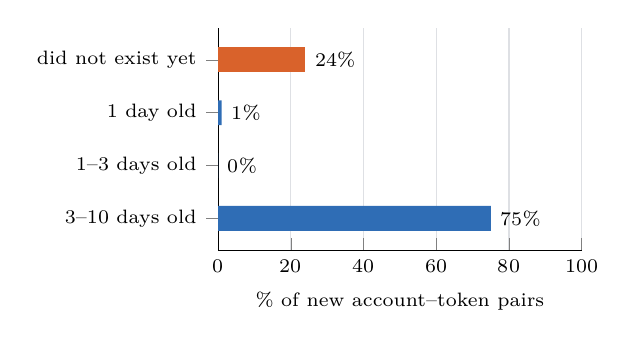
\begin{tikzpicture}
        \begin{axis}[
          width=6.2cm,height=4.4cm, xbar, bar width=9pt, xmin=0, xmax=100, bar shift=0pt,
          symbolic y coords={old,mid,young,none},
          yticklabels={{3--10 days old},{1--3 days old},{1 day old},{did not exist yet}},
          ytick={old,mid,young,none}, y tick label style={font=\scriptsize,align=right},
          xlabel={\% of new account--token pairs}, label style={font=\scriptsize}, tick label style={font=\scriptsize},
          nodes near coords={\pgfmathprintnumber{\pgfplotspointmeta}\%}, nodes near coords style={font=\scriptsize},
          axis lines*=left, enlarge y limits=0.2, xmajorgrids, grid style={grey!25},
        ]
          \addplot[fill=blue,draw=none] coordinates {(75,old)(0,mid)(1,young)};
          \addplot[fill=orange,draw=none] coordinates {(24,none)};
        \end{axis}
      \end{tikzpicture}
      \par\scriptsize\color{grey} The two days after day 10, 24{,}583 pairs.
    \end{column}
    \begin{column}{0.44\textwidth}
      \small
      \textbf{1. Cold start.} 15--25\% of the target tokens did not exist at time $t$. No model of past trades can list them.
      \par\medskip
      \textbf{2. Bimodal adoption.} Tokens are picked up at launch, or once established; little in between.
      \par\medskip
      \textbf{3. Weakest where personalization should help.} Baseline recall@10: 0.18 for accounts with 1--4 tokens, \alert{0.12} for accounts with 5 or more.
    \end{column}
  \end{columns}
\end{frame}

\begin{frame}{Evaluation protocol and the success criterion}
  \small
  \begin{columns}[T]
    \begin{column}{0.5\textwidth}
      \textbf{At every evaluation point}
      \begin{enumerate}
        \item fit every model on the history only;
        \item for each account, score \emph{all} tokens, remove its own, keep 10;
        \item score the lists against the next 2 days.
      \end{enumerate}
      \textbf{Then compare with the baseline, paired by point:}
      \begin{itemize}
        \item mean difference, bootstrap interval over points;
        \item points won: 12 of 14 needed (sign test, 5\%);
        \item also by history size, and without the most popular tokens \cite{cremonesi2010}.
      \end{itemize}
    \end{column}
    \begin{column}{0.46\textwidth}
      \centering
      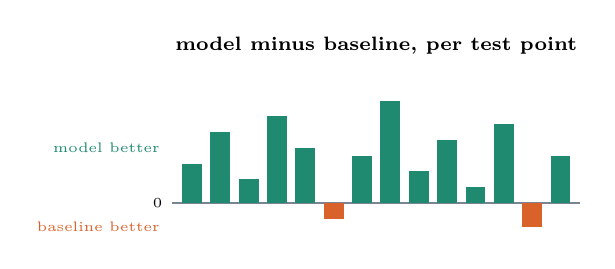
\begin{tikzpicture}[x=0.36cm,y=1cm]
        \node[font=\scriptsize\bfseries] at (7.5,2.0) {model minus baseline, per test point};
        \draw[grey] (0.3,0) -- (14.7,0);
        \foreach \i/\v in {1/0.5,2/0.9,3/0.3,4/1.1,5/0.7,6/-0.2,7/0.6,8/1.3,9/0.4,10/0.8,11/0.2,12/1.0,13/-0.3,14/0.6} {
          \ifdim\v pt<0pt \fill[orange] (\i-0.35,0) rectangle (\i+0.35,\v);
          \else \fill[teal] (\i-0.35,0) rectangle (\i+0.35,\v); \fi
        }
        \node[font=\tiny,anchor=east] at (0.3,0) {0};
        \node[font=\tiny,teal,anchor=east] at (0.2,0.7) {model better};
        \node[font=\tiny,orange,anchor=east] at (0.2,-0.3) {baseline better};
      \end{tikzpicture}
      \par\scriptsize\color{grey} Schematic only. No model results exist yet.
    \end{column}
  \end{columns}
  \takeaway{Fixed in advance: success = higher mean recall@10 than the baseline on the 14 test points, with a bootstrap interval of the paired difference that excludes zero.}
\end{frame}

% ===========================================================================
\section{The proposed method}

\begin{frame}{Stage 1: item-based nearest neighbours \cite{sarwar2001}}
  \begin{columns}[T]
    \begin{column}{0.46\textwidth}
      \small
      \textbf{Idea:} two tokens are similar if the \emph{same accounts} trade them.
      Recommend tokens similar to the account's own.
      \par\smallskip
      $U_i$ = accounts that traded token $i$; $H_u$ = tokens of account $u$.
      \[
        s_{ij} = \frac{|U_i \cap U_j|}{\sqrt{|U_i|\,|U_j|} + \lambda}
        \qquad
        r_{ui} = \sum_{j \in H_u} s_{ji}
      \]
      \begin{itemize}\footnotesize
        \item $\lambda$ (shrinkage) distrusts tokens with few accounts.
        \item Keep only the $k$ most similar tokens per token.
        \item Works from \textbf{one token} of history.
      \end{itemize}
    \end{column}
    \begin{column}{0.5\textwidth}
      \centering\footnotesize
      \textbf{Toy example} (5 accounts, $\lambda=0$)
      \par\smallskip
      \begin{tabular}{@{}lcccc@{}}
        \toprule
        & PEPE & SHIB & LINK & AAVE \\
        \midrule
        A & \textcolor{blue}{$\blacksquare$} & \textcolor{blue}{$\blacksquare$} & & \\
        B & \textcolor{blue}{$\blacksquare$} & \textcolor{blue}{$\blacksquare$} & & \\
        C & \textcolor{orange}{$\blacksquare$} & ? & ? & ? \\
        D & & & \textcolor{blue}{$\blacksquare$} & \textcolor{blue}{$\blacksquare$} \\
        E & & \textcolor{blue}{$\blacksquare$} & \textcolor{blue}{$\blacksquare$} & \\
        \bottomrule
      \end{tabular}
      \par\medskip
      Account C has only PEPE.
      \par\smallskip
      $s_{\text{PEPE,SHIB}} = \dfrac{2}{\sqrt{3\cdot 3}} = 0.67 \qquad s_{\text{PEPE,LINK}} = 0$
      \par\smallskip
      $\Rightarrow$ recommend \textbf{SHIB} to C.
    \end{column}
  \end{columns}
  \takeaway{Combined with popularity as $w\,\tilde p_i + (1-w)\,\tilde r_{ui}$. With $w=1$ this \emph{is} the baseline, so the baseline is a special case.}
\end{frame}

\begin{frame}{Stage 2: a learned ranker on top \cite{covington2016,burges2010}}
  \centering
  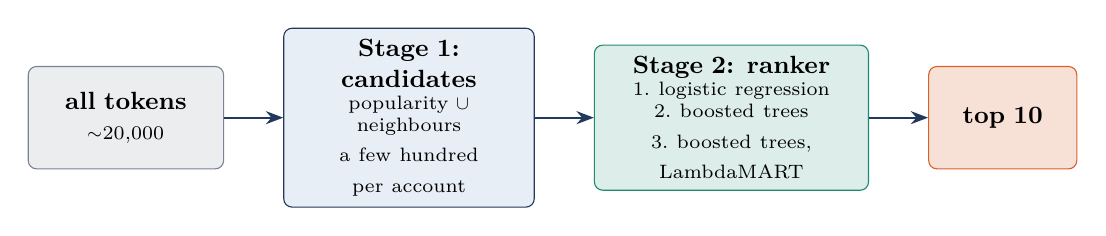
\begin{tikzpicture}[node distance=0.8cm]
    \node[box,fill=grey!15,draw=grey,minimum height=1.3cm,text width=2.2cm] (all) {\textbf{all tokens}\\ \scriptsize $\sim$20{,}000};
    \node[box,right=0.75cm of all,minimum height=1.3cm,text width=2.9cm] (s1) {\textbf{Stage 1: candidates}\\ \scriptsize popularity $\cup$ neighbours\\ a few hundred per account};
    \node[box,right=0.75cm of s1,fill=teal!15,draw=teal,minimum height=1.3cm,text width=3.2cm] (s2) {\textbf{Stage 2: ranker}\\ \scriptsize 1.\ logistic regression\\ 2.\ boosted trees\\ 3.\ boosted trees, LambdaMART};
    \node[box,right=0.75cm of s2,fill=orange!20,draw=orange,minimum height=1.3cm,text width=1.6cm] (out) {\textbf{top 10}};
    \draw[arr] (all) -- (s1); \draw[arr] (s1) -- (s2); \draw[arr] (s2) -- (out);
  \end{tikzpicture}
  \vspace{6pt}
  \begin{columns}[T]
    \begin{column}{0.48\textwidth}
      \small
      \textbf{One training row} = (point, account, candidate token).
      Label 1 if the account trades it for the first time in the next two days.
      \par\medskip
      \textbf{Features} (all from the history): popularity at several time scales, neighbour scores, account history size, token age and early activity.
    \end{column}
    \begin{column}{0.48\textwidth}
      \small
      \textbf{Guarding against overfitting}
      \begin{itemize}
        \item simplest model first
        \item trained on Dev A only (10 points)
        \item validated on held-out points
        \item compared with the best \emph{fixed} combination, not only the baseline
      \end{itemize}
    \end{column}
  \end{columns}
\end{frame}

\begin{frame}{The three core problems of the project}
  \begin{columns}[T]
    \begin{column}{0.32\textwidth}
      \begin{block}{\faUser\ 1. Short histories}
        \small
        The typical account has one token.
        \par\smallskip
        \textbf{Question:} what do neighbours add to popularity?
      \end{block}
    \end{column}
    \begin{column}{0.32\textwidth}
      \begin{block}{\faClock[regular]\ 2. Time weighting}
        \small
        Interest moves fast; the baseline swings 0.11--0.20.
        \par\smallskip
        \textbf{Question:} how much should old trades count?
      \end{block}
    \end{column}
    \begin{column}{0.32\textwidth}
      \begin{block}{\faSeedling\ 3. Cold start}
        \small
        15--25\% of targets did not exist at time $t$.
        \par\smallskip
        \textbf{Question:} how much is reachable with refreshed lists?
      \end{block}
    \end{column}
  \end{columns}
  \takeaway{Each problem enters the ranker as a group of features. Removing one group at a time (ablation) measures what it contributes.}
\end{frame}

% ===========================================================================
\section{Work plan, risks, limitations}

\begin{frame}{Work packages}
  \centering
  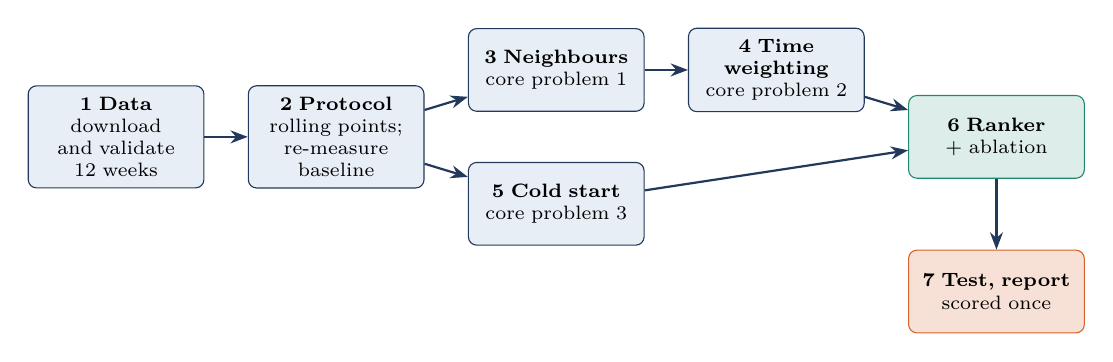
\begin{tikzpicture}[node distance=0.55cm and 0.55cm, wp/.style={box,text width=1.95cm,minimum height=1.05cm,font=\scriptsize}]
    \node[wp] (w1) {\textbf{1 Data}\\download and validate 12 weeks};
    \node[wp,right=of w1] (w2) {\textbf{2 Protocol}\\rolling points; re-measure baseline};
    \node[wp,right=of w2,yshift=0.85cm] (w3) {\textbf{3 Neighbours}\\core problem 1};
    \node[wp,right=of w3] (w4) {\textbf{4 Time weighting}\\core problem 2};
    \node[wp,right=of w2,yshift=-0.85cm] (w5) {\textbf{5 Cold start}\\core problem 3};
    \node[wp,right=of w4,yshift=-0.85cm,fill=teal!15,draw=teal] (w6) {\textbf{6 Ranker}\\+ ablation};
    \node[wp,below=0.9cm of w6,fill=orange!20,draw=orange] (w7) {\textbf{7 Test, report}\\scored once};
    \draw[arr] (w1) -- (w2);
    \draw[arr] (w2) -- (w3); \draw[arr] (w2) -- (w5);
    \draw[arr] (w3) -- (w4);
    \draw[arr] (w4) -- (w6); \draw[arr] (w5) -- (w6);
    \draw[arr] (w6) -- (w7);
  \end{tikzpicture}
  \vspace{4pt}
  \begin{itemize}\small
    \item Every step is judged against the step before it, and always against the fixed baseline.
    \item Optional if time allows: matrix factorization (iALS) \cite{rendle2021} and EASE \cite{steck2019} as references.
  \end{itemize}
\end{frame}

\begin{frame}{Risks and limitations, stated plainly}
  \small
  \begin{columns}[T]
    \begin{column}{0.49\textwidth}
      \textbf{Risks}
      \begin{itemize}
        \item \textbf{The method may not beat popularity.} This is common in the literature \cite{li2021}. A clean null result on 14 test points is still a result.
        \item \textbf{Day-to-day effects may hide model effects.} Hence many points and paired comparisons.
        \item \textbf{The ranker may overfit} 10 market situations. Hence simple models and held-out points.
      \end{itemize}
    \end{column}
    \begin{column}{0.49\textwidth}
      \textbf{Limitations of the evidence so far}
      \begin{itemize}
        \item Two weeks, one market phase; only the baseline has results.
        \item One account $\neq$ one person; bots are not removed.
        \item Only Uniswap V2/V3-style pools.
      \end{itemize}
      \textbf{Use and harm.} Recommending speculative tokens is not obviously good. We treat this as a study of trading behaviour and of evaluation, not as a product.
    \end{column}
  \end{columns}
\end{frame}

\begin{frame}{Summary}
  \small
  \renewcommand{\arraystretch}{1.3}
  \begin{tabularx}{\textwidth}{@{}>{\bfseries}p{3.3cm}>{\raggedright\arraybackslash}X@{}}
    \toprule
    Task & For each account, rank the tokens it never traded; a hit is a first trade in the next 2 days. \\
    Data & Uniswap-style swaps on Ethereum. Studied: 14 days, 2.71 M swaps. Planned: 12 earlier weeks. \\
    Split & One global timeline. Dev A tunes, Dev B selects, 14 test points scored once. \\
    Baseline & 10 most popular tokens: recall@10 = 0.155 (0.11--0.20 by day). \\
    Method & Item neighbours + popularity, then a learned ranker. \\
    Core problems & Short histories, time weighting, cold start. \\
    Success & Higher mean recall@10 on test, with a paired interval excluding zero. \\
    \bottomrule
  \end{tabularx}
  \vspace{8pt}
  \begin{center}\Large\color{navy} Thank you. Questions?\end{center}
\end{frame}

% ---------------------------------------------------------------------------
\begin{frame}[allowframebreaks,t]{References}
  \setbeamertemplate{bibliography item}{\insertbiblabel}
  \begin{thebibliography}{Covington 2016}
    \scriptsize
    % The 21 references of the project plan. Shared by both decks.
% \bibitem[label]{key}: the label is what \cite prints on the slides.
\bibitem[Hu 2008]{hu2008} Y.~Hu, Y.~Koren, C.~Volinsky. Collaborative filtering for implicit feedback datasets. \emph{ICDM}, 2008.
\bibitem[Rendle 2009]{rendle2009} S.~Rendle, C.~Freudenthaler, Z.~Gantner, L.~Schmidt-Thieme. BPR: Bayesian personalized ranking from implicit feedback. \emph{UAI}, 2009. arXiv:1205.2618.
\bibitem[Sarwar 2001]{sarwar2001} B.~Sarwar, G.~Karypis, J.~Konstan, J.~Riedl. Item-based collaborative filtering recommendation algorithms. \emph{WWW}, 2001.
\bibitem[Cremonesi 2010]{cremonesi2010} P.~Cremonesi, Y.~Koren, R.~Turrin. Performance of recommender algorithms on top-N recommendation tasks. \emph{RecSys}, 2010.
\bibitem[Steck 2019]{steck2019} H.~Steck. Embarrassingly shallow autoencoders for sparse data. \emph{WWW}, 2019. arXiv:1905.03375.
\bibitem[Hidasi 2016]{hidasi2016} B.~Hidasi, A.~Karatzoglou, L.~Baltrunas, D.~Tikk. Session-based recommendations with recurrent neural networks. \emph{ICLR}, 2016. arXiv:1511.06939.
\bibitem[Dacrema 2019]{dacrema2019} M.~F.~Dacrema, P.~Cremonesi, D.~Jannach. Are we really making much progress? A worrying analysis of recent neural recommendation approaches. \emph{RecSys}, 2019. arXiv:1907.06902.
\bibitem[Rendle 2020]{rendle2020} S.~Rendle, W.~Krichene, L.~Zhang, J.~Anderson. Neural collaborative filtering vs.\ matrix factorization revisited. \emph{RecSys}, 2020. arXiv:2005.09683.
\bibitem[Rendle 2021]{rendle2021} S.~Rendle, W.~Krichene, L.~Zhang, Y.~Koren. Revisiting the performance of iALS on item recommendation benchmarks. arXiv:2110.14037, 2021.
\bibitem[Anelli 2022]{anelli2022} V.~W.~Anelli, A.~Bellogín, T.~Di~Noia, D.~Jannach, C.~Pomo. Top-N recommendation algorithms: a quest for the state-of-the-art. \emph{UMAP}, 2022. arXiv:2203.01155.
\bibitem[Ludewig 2018]{ludewig2018} M.~Ludewig, D.~Jannach. Evaluation of session-based recommendation algorithms. \emph{User Modeling and User-Adapted Interaction}, 2018. arXiv:1803.09587.
\bibitem[Li 2021]{li2021} M.~Li, S.~Jullien, M.~Ariannezhad, M.~de~Rijke. A next basket recommendation reality check. arXiv:2109.14233, 2021.
\bibitem[Ji 2020a]{ji2020pop} Y.~Ji, A.~Sun, J.~Zhang, C.~Li. A re-visit of the popularity baseline in recommender systems. \emph{SIGIR}, 2020. arXiv:2005.13829.
\bibitem[Ji 2020b]{ji2020leak} Y.~Ji, A.~Sun, J.~Zhang, C.~Li. A critical study on data leakage in recommender system offline evaluation. arXiv:2010.11060, 2020.
\bibitem[Meng 2020]{meng2020} Z.~Meng, R.~McCreadie, C.~Macdonald, I.~Ounis. Exploring data splitting strategies for the evaluation of recommendation models. \emph{RecSys}, 2020. arXiv:2007.13237.
\bibitem[Krichene 2020]{krichene2020} W.~Krichene, S.~Rendle. On sampled metrics for item recommendation. \emph{KDD}, 2020.
\bibitem[Schein 2002]{schein2002} A.~Schein, A.~Popescul, L.~Ungar, D.~Pennock. Methods and metrics for cold-start recommendations. \emph{SIGIR}, 2002.
\bibitem[Choi 2024]{choi2024} Choi et al. A recommender system for NFT collectibles with item feature. arXiv:2403.18305, 2024.
\bibitem[Li 2023]{nftmine2023} S.~Li, Y.~Jin, P.-L.~Hsu, Y.-S.~Luo. NFT.mine: an xDeepFM-based recommender system for non-fungible token (NFT) buyers. arXiv:2306.03942, 2023.
\bibitem[Burges 2010]{burges2010} C.~J.~C.~Burges. From RankNet to LambdaRank to LambdaMART: an overview. Microsoft Research Tech.\ Report MSR-TR-2010-82, 2010.
\bibitem[Covington 2016]{covington2016} P.~Covington, J.~Adams, E.~Sargin. Deep neural networks for YouTube recommendations. \emph{RecSys}, 2016.

  \end{thebibliography}
\end{frame}

\end{document}
